\documentclass[11pt]{article}
\usepackage[margin=1in]{geometry}
\usepackage[T1]{fontenc}
\usepackage{lmodern}
\usepackage{amsmath}
\usepackage{graphicx}
\usepackage{tikz}
\usetikzlibrary{arrows.meta,calc,positioning,shapes.geometric}
\usepackage{pgfplots}
\pgfplotsset{compat=1.18}
\usepackage[colorlinks=true,linkcolor=blue,citecolor=blue,urlcolor=blue]{hyperref}
\usepackage[nameinlink,noabbrev]{cleveref}

\title{TikZ and PGFPlots Conversion Stress Paper}
\author{Stage Two Corpus}
\date{}

\begin{document}
\maketitle

\section{Purpose}

This short paper isolates two vector graphics cases that are common in technical manuscripts. The first figure uses a TikZ node-and-arrow diagram with styled shapes and relative positioning. The second figure uses a \texttt{pgfplots} axis with computed curves. A converter that depends only on abstract syntax must decide whether these environments require compilation to an external image.

\begin{figure}[tbp]
\centering
\resizebox{\linewidth}{!}{%
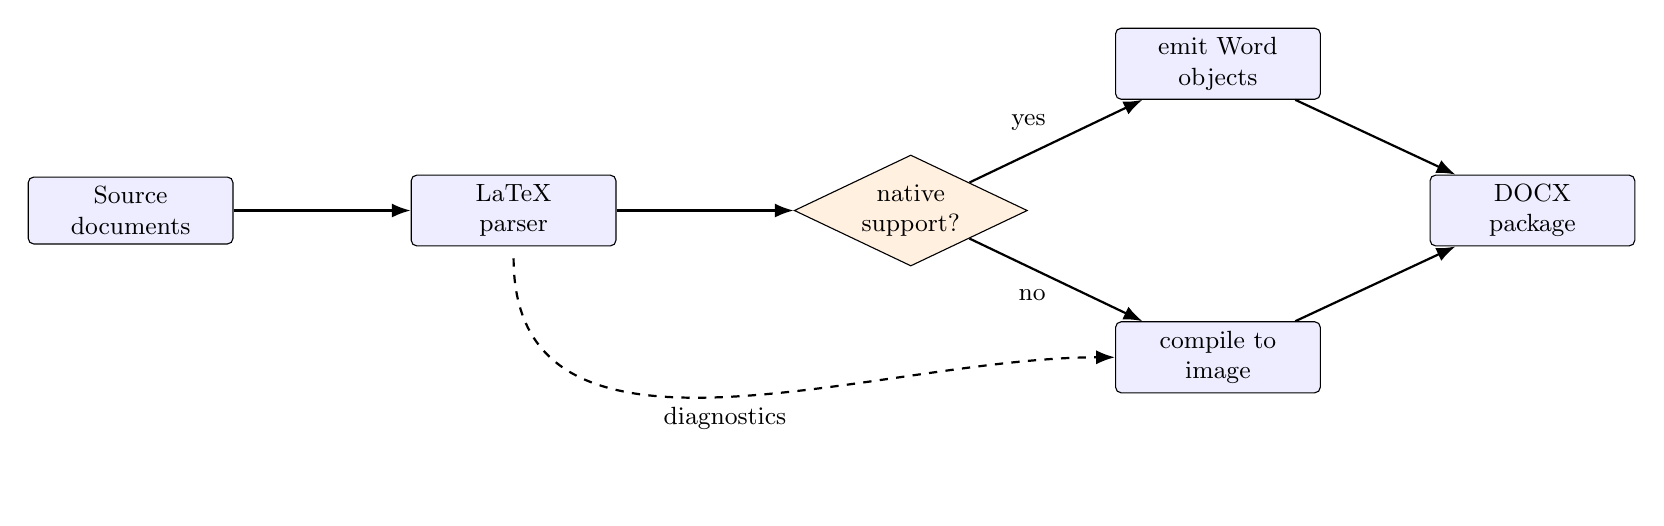
\begin{tikzpicture}[
  node distance=2.25cm,
  every node/.style={font=\small},
  block/.style={draw, rounded corners=2pt, align=center, minimum width=2.6cm, minimum height=0.85cm, fill=blue!7},
  decision/.style={draw, diamond, aspect=2.1, align=center, inner sep=1.5pt, fill=orange!12},
  arrow/.style={-{Latex[length=2.4mm]}, thick}
]
\node[block] (source) {Source\\documents};
\node[block, right=of source] (parser) {LaTeX\\parser};
\node[decision, right=of parser] (branch) {native\\support?};
\node[block, above right=1.05cm and 1.85cm of branch] (native) {emit Word\\objects};
\node[block, below right=1.05cm and 1.85cm of branch] (render) {compile to\\image};
\node[block, right=5.1cm of branch] (docx) {DOCX\\package};

\draw[arrow] (source) -- (parser);
\draw[arrow] (parser) -- (branch);
\draw[arrow] (branch) -- node[above left]{yes} (native);
\draw[arrow] (branch) -- node[below left]{no} (render);
\draw[arrow] (native) -- (docx);
\draw[arrow] (render) -- (docx);
\draw[arrow, dashed] ($(parser.south)+(0,-0.15)$) to[out=-90,in=180] node[below]{diagnostics} (render.west);
\end{tikzpicture}
}
\caption{A vector node-and-arrow workflow diagram drawn directly with TikZ.}
\label{fig:tikz-workflow}
\end{figure}

\Cref{fig:tikz-workflow} contains shapes, custom arrows, a dashed diagnostic path, and positional arithmetic. These constructs are intentionally chosen because they are difficult to represent through a Word drawing model without executing the TeX graphics layer.

\begin{figure}[tbp]
\centering
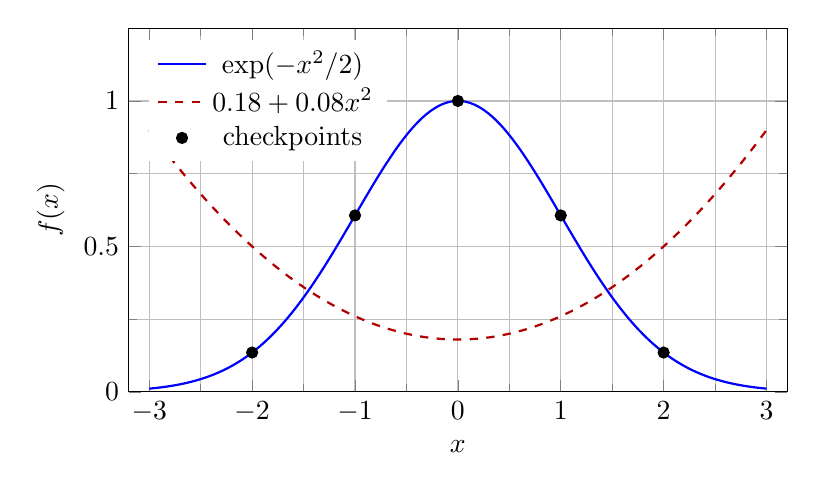
\begin{tikzpicture}
\begin{axis}[
  width=0.82\linewidth,
  height=6.2cm,
  xlabel={$x$},
  ylabel={$f(x)$},
  xmin=-3.2,
  xmax=3.2,
  ymin=0,
  ymax=1.25,
  grid=both,
  minor tick num=1,
  legend style={draw=none, fill=white, at={(0.03,0.97)}, anchor=north west},
  samples=161
]
\addplot[blue, thick, domain=-3:3] {exp(-x^2/2)};
\addlegendentry{$\exp(-x^2/2)$}
\addplot[red!70!black, dashed, thick, domain=-3:3] {0.18 + 0.08*x^2};
\addlegendentry{$0.18+0.08x^2$}
\addplot[black, mark=*, only marks] coordinates {(-2,0.1353) (-1,0.6065) (0,1) (1,0.6065) (2,0.1353)};
\addlegendentry{checkpoints}
\end{axis}
\end{tikzpicture}
\caption{A PGFPlots axis with a smooth curve, a comparison curve, and marked checkpoints.}
\label{fig:pgfplots-curve}
\end{figure}

The plotted axis in \cref{fig:pgfplots-curve} tests a different part of the graphics stack. Tick labels, legends, grid lines, computed functions, and explicit coordinates must travel together for the figure to remain intelligible.

\end{document}
